\part{Teoria Atômica I}

% Slide 8
\section*{História}

% Grécia Antiga
\begin{sectionBox}1m{Do grego: Átomos} % άτομο

    No \(5^o\) Século A.C o filosofo Leucippus de Miletus originou a filosofia atômica, seu discípulo Democritus de Abdera nomeou átomo significando literalmente indivisível, e caracterizou os átomos por possuirem tamanhos e formas diferentes atribuindo a matéria que eles formam suas características.

    A filosofia atômica nunca foi aceita por Aristotles e como sua filosofia deu origem a igreja cristã na europa, a igreja perseguiu aqueles que iam contra a filosofia aristotélica, atrasando bastante o desenvolvimento da teoria atômica.

\end{sectionBox}% John Dalton



% Dalton
\begin{sectionBox}1m{Teoria Atómica de Dalton}

    Apenas no século 19 d.c a teoria atómica foi retomada com a publicação do livro \textit{A New System of Chemical Philosophy} de John Dalton com base no princípio da conservação de massa em reações químicas de Lavoisier, elevando o conceito filosófico de átomo para uma teoria química. Dentre os conteúdos de sua publicação se discutiam o seguinte:

    \begin{sectionBox}2{Postulados}
        \begin{enumerate}
            \item Elementos consistem de minusculas particulas sem carga, indestrutíveis e indivisíveis;
            \item Todos os átomos do mesmo elemento são iguais, diferentes elementos possuem diferentes tipos de átomos;
            \item Átomos não são nem criados nem destruídos;
            \item Diferentes átomos podem se juntar em simples proporções para formar ``átomos compostos''.
        \end{enumerate}
    \end{sectionBox}

\end{sectionBox}



% Slide 11
% J. J. Thompson
\begin{sectionBox}1{J. J. Thomson: modelo pudim de passas}

    \begin{sectionBox}2{Pretexto: Experimentos com ampola de Crooks}

        Ampolas alongadas e vedadas onde se podia inserir gases e reduzir sua pressão com uma bomba de vácuo, alem de possuir um cátodo e um anodo de pilhas em cada uma das suas extremidades.

        Ao diminuir a pressão á 10\,\unit{\milli\meter\ch{Hg}} no interior de uma ampola preenchida com hidrogênio uma luz rosa passou a ser emitida pela ampola.

        ...

        % profit

    \end{sectionBox}

    \begin{itemize}
        \item átomos possuem pequenas partículas carregadas negativamente (elétrons)
        \item núcleo positivo constitui praticamente toda a massa do átomo
    \end{itemize}

\end{sectionBox}



% Rutherford
\begin{sectionBox}1{Experimento da folha de ouro de Rutherford}

    Bloco contendo Rádio emissor de partículas \alpha (positivas) que colidem com uma fina lamina de ouro, verificando o desvio das partículas \alpha que poderiam apenas ser explicadas pela interação elétrica com o campo gerado pelo núcleo dos átomos de ouro, que para possuir um campo suficientemente forte precisa ser pequeno.

    Para que o núcleo seja pequeno, os elétrons tem que orbitar ao seu redor, e se esse for o caso pelas leis de Maxuel partículas carregadas em aceleração perdem energia em forma de ondas eletromagnéticas e os elétrons se colidiria com o núcleo causando a % <nome bnt p colizão eletron e nucleo>
    em alguns milésimos o que obviamente não ocorre.

    A conclusão desse experimento contraria Maxuel, e por isso Rutherford descontinuou seus estudos atômicos.

\end{sectionBox}

% Hantaro Nagaoka...primeira proposição do modelo planetário

% Teoria dos orbitais de Bohr
\begin{sectionBox}1m{Teoria orbital de Bohr}

    Usando o ``\textit{insight}'' de Rutherford

    % Postulados de Bohr
    \begin{enumerate}
        \item Eletrons existem em estados estacionários
        \item Qualquer variação do eletron no estado estacionario implica em absorção e emição de ondas eletromagnéticas
        \item momento angular do eletron é quantizado ou \( L = |m_e\,\vec{v}\times\vec{r}| = n\,K \quad\forall\,n\in\mathbb{K} \)
            onde \(k=h/2\,\pi\)
    \end{enumerate}

    \begin{center}
        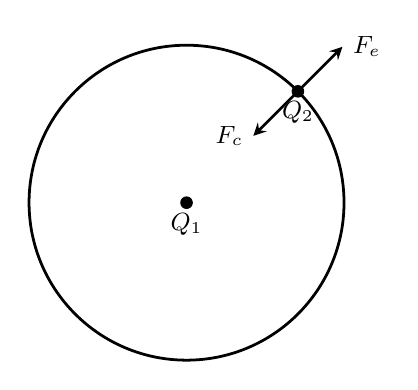
\begin{tikzpicture}[
            scale=1, font=\small, align=center, line width=1
        ]
            \draw(0,0) circle (2);

            % Q1
            \fill(0,0) circle (.08) node[below]{\(Q_1\)};

            % Q2
            \coordinate(q2) at (45:2);
            \fill(q2) circle (.08) node[below]{\(Q_2\)};

            \draw[-stealth] (q2) --  +(45:0.8) node[right]{\(F_e\)};
            \draw[-stealth] (q2) -- +(225:0.8) node[left ]{\(F_c\)};

        \end{tikzpicture}
    \end{center}

    % Slide 23
    \begin{sectionBox}*2{Raio da orbita}
        \begin{flalign*}
            &
                m_e\,v^2/r = F_c = F_e = \frac{e^2}{4\,\pi\,\varepsilon_0\,r^2}
            \land
                m_e\,v\,r = \frac{n\,h}{2\,\pi}
            \implies &\\&
            \implies
                r
            =   \cfrac
                    {e^2}
                    {
                        4\,\pi\,\varepsilon_0\,m_e
                    \,  \left(
                            \frac{n\,h}{2\,\pi\,m_e\,r}
                        \right)^2
                    }
            \implies
                r
            =   \frac{\varepsilon_0\,n^2\,h^2}{e^2\,\pi\,m_e}
            &
        \end{flalign*}
    \end{sectionBox}

    \begin{sectionBox}*2{velocidade do elétron}
        \begin{flalign*}
            &
                m_e\,v\,r
            =   \frac{n\,h}{2\,\pi}
            \implies
                v
            =   \cfrac
                    {n\,h}
                    {
                        2\,\pi\,m_e
                    \,  \left(
                            \frac{\varepsilon_0\,n^2\,h^2}{e^2\,\pi\,m_e}
                        \right)
                    }
            =   \frac{e^2}{2\,\varepsilon_0\,n\,h}
            &
        \end{flalign*}
    \end{sectionBox}

    \begin{sectionBox}*2{Energia Cinética}
        \begin{flalign*}
            &
                E_c
            =   \frac{m_e\,v^2}{2}
            =   \frac{m_e}{2}
            \,  \left(
                    \frac{e^2}{2\,\varepsilon_0\,n\,h}
                \right)^2
            =   \cfrac
                    {
                        \left(
                            \frac{m_e\,e^4}{8\,\varepsilon_0^2\,h^2}
                        \right)
                    }
                    {n^2}
            =   k/n^2
            &
        \end{flalign*}
    \end{sectionBox}

    \begin{sectionBox}*2{Energia Potencial}
        \begin{flalign*}
            &
                E_p
            =   \frac{-e^2}{4\,\pi\,\varepsilon_0\,r}
            =   \cfrac
                    {-e^2}
                    {
                        4\,\pi\,\varepsilon_0
                    \,  \left(
                            \frac{\varepsilon_0\,n^2\,h^2}{e^2\,\pi\,m_e}
                        \right)
                    }
            =   \frac{-2\,m_e\,e^4}{8\,\varepsilon_0^2\,n^2\,h^2}
            =   -2\,k/n^2
            &
        \end{flalign*}
    \end{sectionBox}

    % Energia total
    \begin{sectionBox}*2{Energia total}
        \begin{flalign*}
            &
                E_t
            =   E_c + E_p
            =   k/n^2 - 2\,k/n^2
            =   -k/n^2
            &
        \end{flalign*}
    \end{sectionBox}

    % k
    \begin{sectionBox}*2{k}
        \begin{flalign*}
            &
                k
            =   \frac{m_e\,e^4}{8\,\varepsilon_0^2\,h^2}
            = &\\&
            =   \frac
                    {
                        9.10938356*10^{-31}\,\unit{\kilo\gram}
                    *   (1.60217662*10^{-19}\,\unit{\coulomb})^4
                    }
                    {
                        8
                    *   (8.8541878128*10^{-12}\,\unit{\farad\per\metre})^2
                    *   (6.62607015*10^{-34}\,\unit{\joule\per\hertz})^2
                    }
            \cong &\\&
            \cong
                2.179872251033439*10^{-18}\,\unit{\frac{\kilo\gram\coulomb^4\metre^2\hertz^2}{\farad^2\joule^2}}
            \cong
                \qty [round-precision=5, exponent-to-prefix=false]
                    {2.179872251033439e-18}{\frac{\kilo\gram\coulomb^4\metre^2\hertz^2}{\farad^2\joule^2}}
            &
        \end{flalign*}
    \end{sectionBox}

\end{sectionBox}
